%%%%
% Consiglio la visione dei seguenti tutorial:
% - https://www.youtube.com/watch?v=ihxSUsJB_14
% - https://www.youtube.com/watch?v=XTFWaV55uDo
%%%%
\documentclass[12pt,a4paper,openright,twoside]{book}
\usepackage[utf8]{inputenc}
\usepackage{amsmath}
\usepackage{algorithmic}
\usepackage{amssymb}
\usepackage{algorithm}
\usepackage{algpseudocode}


\newcommand{\thesislang}{english} % commentare in caso di tesi in italiano
\usepackage{thesis-style}
% version
\newcommand{\versionmajor}{0}
\newcommand{\versionminor}{1}
\newcommand{\versionpatch}{2}
\newcommand{\version}{\versionmajor.\versionminor.\versionpatch}
\typeout{Document version: \version}

\begin{document}
	
\frontmatter

% ! TeX root = thesis-main.tex
\title{Title}
\author{Candidate Name Here}
\date{\today}

\newgeometry{margin=0.8in}
\begin{titlepage}
	\begin{center}
		% \vspace*{0.2cm}
		
		\large
		\textbf{ALMA MATER STUDIORUM -- UNIVERSITÀ DI BOLOGNA \\ CAMPUS DI CESENA}
		\\
		\noindent\hrulefill
		\vspace{0.4cm}
		
		\Large
		Scuola di Ingegneria e Architettura \\
		Corso di Laurea Magistrale in Ingegneria e Scienze Informatiche
		
		\Huge
		\vspace{4cm}
		\textbf{
			Fair-by-design algorithm for access to education
		}
		
		\large
		\vspace{1cm}
		Tesi di laurea in 
		\\
		\textsc{Intelligent System Engineering}
		
		\vspace{5.5cm}
		\begin{minipage}[t]{0.64\textwidth}
			\begin{flushleft}
				\textit{Relatore} 
				\\ 
				\textbf{Prof.} \textbf{Giovanni Ciatto}
				\\
				\vspace{0.4cm}
				\textit{Correlatore} 
				\\
				\textbf{Prof.} \textbf{Roberta Calegari}
				\textbf{Prof.} \textbf{Andre Omicini}
			\end{flushleft}
		\end{minipage}
		\begin{minipage}[t]{0.34\textwidth}
			\begin{flushright}
				\textit{Candidato} 
				\\ 
				\textbf{Antonio Iannotta}
			\end{flushright}
		\end{minipage}\\
		
		\vfill
		\noindent\hrulefill
		\vspace{0.3cm}
		\Large
		
		IV Sessione di Laurea
		\\
		Anno Accademico 2022-2023
	\end{center}
\end{titlepage}
\restoregeometry


\begin{abstract}	
Nowdays a lot of companies and social entities are wondering about the implications of Artificial Intelligence usages in the daily life of people, with a 
huge interests for the implications in discriminations that may occour using these systems. \\
A lot of methodologies in several fields like computer science, statistics and social sciences have been formalized in order to 
afford the problem of the fairness in social systems and this problem is being dealt with during the development of the modern AI systems. \\
In this work we propose several methods that have been developed considering fairness from the design phase, that's why they are called \emph{fair-by-design-method}
In order to develop these methods we used well-known Python libraries such as \emph{Pandas}, \emph{Sci-kit-learn} and other libraries implemented by ourselves.
We begun our work with mitigation techniques in fairness, also known as pre-processing techniques.
Our work has been evaluated exploiting a real-world dataset on the education on Canary Island. So we compared the results of the prediction of a certain result for students applying fair-by-design methods and 
the prediction obtained without consider fairness.
\end{abstract}

%\begin{dedication} % this is optional
%Optional. Max a few lines.
%\end{dedication}

\begin{acknowledgements} % this is optional
Never too far down, to come back
\end{acknowledgements}

%----------------------------------------------------------------------------------------
\tableofcontents   
\listoffigures     % (optional) comment if empty
\lstlistoflistings % (optional) comment if empty
%----------------------------------------------------------------------------------------

\mainmatter

%----------------------------------------------------------------------------------------
\chapter{\introductionname}
\label{chap:introduction}
%----------------------------------------------------------------------------------------

Write introduction here.

%
\paragraph{Thesis Structure.} % Optional paragraph title
%

(This is optional an optional paragraph.)
%
Accordingly, the reminder of this thesis is structures as follows.
%
\Cref{chap:background} discusses (briefly describe the content of \cref{chap:background}).
%
Describe other chapters here in a similar way.
%
Finally, \Cref{chap:conclusions} concludes this thesis by summarising its main contribution.

%----------------------------------------------------------------------------------------
\chapter{State of the Art} % or Background
\label{chap:background}
%----------------------------------------------------------------------------------------

Write background here.

This section is likely to contain a lot of citations.
%
For instance in \cite{AnzengruberSocInfo2013} the authors propose a novel means for tackling with the problem of preventing bad things from happening.

%----------------------------------------------------------------------------------------
\chapter{Design} % possible chapter for Projects
\label{chap:design}
%----------------------------------------------------------------------------------------
In the subsequent discussion, we will delve into algorithms specifically crafted to address and mitigate fairness concerns. Fairness in algorithms has gained significant attention in recent years due to the realization that traditional computational processes can inadvertently perpetuate biases and disparities. Various approaches, ranging from re-weighting instances to modifying decision boundaries, aim to rectify these issues and promote a more equitable and just application of algorithms across diverse demographics. By exploring these approaches, we aim to shed light on the potential solutions that can contribute to a more inclusive and fair technological landscape.

\section{Conscious fairness through unawareness}

This methodology belongs to the pre-processing techniques to deal with unfairness-issues in a dataset.

The goals of our proposed approach are as follows:
\begin{enumerate}
    \item Make the dataset bias-free by removing both the protected attributes and proxy variables.
    \item Ensure that the algorithm is independent of any specific machine learning models used during the training step.
    \item Extend the approach beyond the removal of only protected attributes to eliminate all other attributes that, according to a certain rule, could indirectly lead to the protected attributes.
\end{enumerate}

Achieving these goals is essential for building a fair and transparent algorithm that is not only effective in removing biases but is also adaptable to different contexts and machine learning models.

\subsection{General Concepts}
Let's consider a dataset \( D \) belonging to \( \mathbb{R}^{n \times m} \) with \( k \) protected variables.

\subsubsection{Formalization of Fairness Evaluation}
We define \textit{fairness\_evaluation} as follows:
\[
\text{fairness\_evaluation}(v_i, Y) = \lambda(v_i, Y) \quad \forall i \in [1, k]
\]

where:
\begin{align*}
v\_i & : \text{ith attribute belonging to the protected variables}, \\
Y & : \text{output column}.
\end{align*}

The fairness function \( \lambda \) evaluates the relationship between a protected attribute \( v_i \) and the output \( Y \), producing a value that represents the level of fairness for that protected attribute.

\subsubsection{Formalization of dataset\_fair}
We define \textit{dataset\_fair} as follows: a dataset \( D \) is considered fair if for every value \( v \) belonging to \textit{fairness\_evaluation}, the following condition holds:
\[ 0.8 \leq v \leq 1.25 \]

\subsection{Utilizing the Apriori Algorithm}
The Apriori algorithm is a powerful tool in association mining, often used for discovering frequent itemsets in transaction databases. In our context, we adapt the Apriori algorithm to identify associations and dependencies between attributes in the dataset. By analyzing the correlations and patterns among attributes, we aim to uncover potential proxies that indirectly lead to sensitive attributes.

To apply the Apriori algorithm, we transform the dataset into a suitable transactional format, where each transaction corresponds to an instance and contains the attributes present in that instance. The algorithm then identifies frequent itemsets, which represent combinations of attributes that occur with high frequency in the dataset.

We interpret these frequent itemsets as potential proxies or indirect indicators of sensitive attributes. By carefully examining and validating these associations, we can make informed decisions about which attributes to remove from the dataset to achieve fairness through unawareness.

\subsubsection{Identifying Proxy Variables with Apriori}

We define \textit{proxy\_detection} as follows: for each antecedent \( A_i \) belonging to the antecedent list \( \mathcal{A} \), for each consequent \( C_j \) belonging to the consequent list \( \mathcal{C} \), and for each protected variable \( V_k \) belonging to the protected variable list \( \mathcal{V} \), \( A_i \) is a proxy if the fairness metric \( \lambda(A_i, C_j) \) is such that:

\[\lambda(A_i, C_j) < 0.8 \quad \text{or} \quad \lambda(A_i, C_j) > 1.25\]

In other words, an antecedent \( A_i \) is considered a proxy if the fairness measure \( \lambda \) between \( A_i \) and a consequent \( C_j \) is outside the acceptable range [0.8, 1.25].

\subsection{Proxy detection only considering variables}
In this section, we delve into the critical task of identifying proxy variables within the dataset. We specifically concentrate on leveraging fairness metrics, normal variables, and protected variables to determine proxies. Proxy variables are indirect indicators or correlates that may indirectly affect sensitive attributes, potentially introducing bias in our dataset. By examining the relationships between these variables and evaluating them based on fairness metrics, we aim to discern which variables exhibit significant associations with the sensitive attributes, leading to their identification as potential proxies. We focus on utilizing fairness metrics to ensure a comprehensive evaluation that considers both the fairness and equity aspects of the dataset, with the ultimate goal of achieving a more equitable and unbiased data representation.

Let us now explore the methodology and approach involved in identifying these crucial proxy variables.

\subsubsection{Proxy detection}
Let's consider the set \( A \), represented as the set of all variables in the dataset excluding the protected variables, and the set \( B \), representing the protected variables.

We define \textit{proxy\_detection} as follows: for every variable \( \text{var} \) belonging to \( A \) and for every protected variable \( \text{var\_protected} \) belonging to \( B \), the variable is a proxy if the fairness metric \( \lambda(\text{var}, \text{var\_protected}) \) satisfies the condition:

\[
\lambda(\text{var}, \text{var\_protected}) < 0.8 \quad \text{or} \quad \lambda(\text{var}, \text{var\_protected}) > 1.25
\]

In other words, a variable \( \text{var} \) is considered a proxy if the fairness measure \( \lambda \) between \( \text{var} \) and a protected variable \( \text{var\_protected} \) falls outside the acceptable range [0.8, 1.25].

\section{Other general concepts}

\subsubsection{Proxy-Free Dataset Function}

Considering the dataset \( D \) belonging to \( \mathbb{R}^{n \times m} \) and \( k \) as the number of identified proxy variables, we define the function \( \text{proxy\_free\_dataset} \) as follows:

\[
\text{proxy\_free\_dataset}: D \times \mathbb{R}^{k \times 1} \rightarrow \mathbb{R}^{n \times (m - k)}
\]

where \( j = m - k \) and \( \text{proxy\_free\_dataset}(D) \) yields a dataset \( \mathbb{R}^{n \times j} \) devoid of the proxy variables, ensuring the removal of any potential indirect indicators that may influence sensitive attributes.

\subsubsection{Protected-Attributes-Free Dataset Function}

Considering the dataset \( D \) belonging to \( \mathbb{R}^{n \times j} \) where j are the columns obtained after the proxy removals and \( k \) as the number of identified protected variables, we define the function \( \text{protected\_attributes\_free\_dataset} \) as follows:

\[
\text{protected\_attributes\_free\_dataset}: D \times \mathbb{R}^{k \times 1} \rightarrow \mathbb{R}^{n \times (j - k)}
\]

where \( p = j - k \) and \( \text{protected\_attributes\_free\_dataset}(D) \) yields a dataset \( \mathbb{R}^{n \times p} \) devoid of the protected variables, ensuring the removal of any potential indirect indicators that may influence sensitive attributes.

\subsection{Pseudocode}
Here's the pseudocode of the algorithm described before. \\

\begin{algorithm}
\caption{Dataset Processing Algorithm}
\begin{algorithmic}[1]
\Procedure{ProcessDataset}{\text{dataset}}
  \While{\textbf{not} \Call{DatasetFair}{$\text{dataset}$} \textbf{or} \text{protected\_attributes in dataset}}
    \State \text{proxies} $\gets$ \Call{ProxyDetection}{$\text{dataset}$}
    \If{\text{proxies is empty}}
      \State $\text{dataset} \gets \text{ProtectedAttributesFreeDataset}(\text{dataset})$
    \Else
      \State $\text{dataset} \gets \text{ProxyFreeDataset}(\text{dataset})$
    \EndIf
  \EndWhile
  \State \textbf{return} \text{dataset}
\EndProcedure
\end{algorithmic}
\end{algorithm}

\begin{figure}
	\centering
	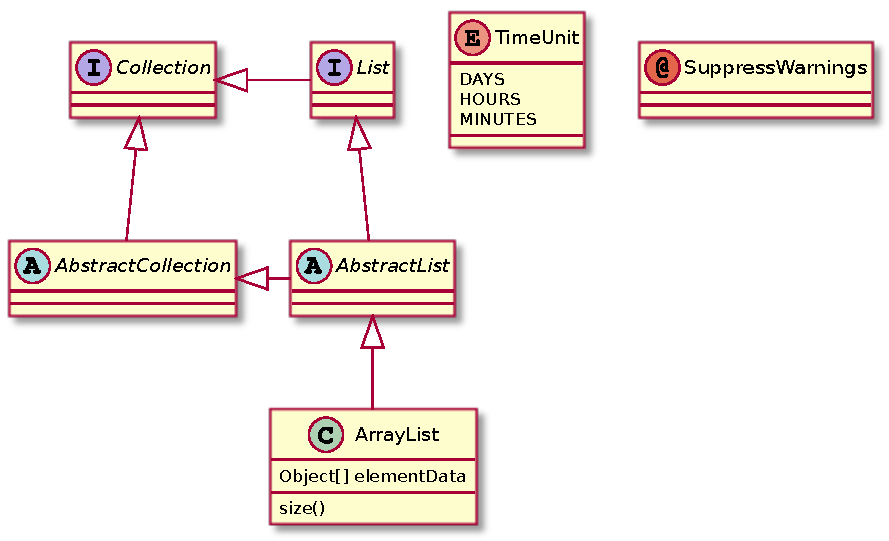
\includegraphics[width=0.5\linewidth]{figures/classes.pdf}
	\caption{A class diagram created with PlantUML}
	\label{fig:classes}
\end{figure}


\section{Fairness through data rebalancing}
chieving fairness in machine learning models is a critical goal to mitigate biases and ensure equitable outcomes across different demographic groups. In many real-world scenarios, datasets are imbalanced, especially concerning sensitive attributes such as race or gender, which can lead to biased predictions. Biased predictions can perpetuate and even exacerbate existing societal inequalities. Addressing this bias and promoting fairness in predictive models is essential for responsible and ethical deployment of machine learning solutions.

This work introduces an innovative algorithm aimed at addressing dataset imbalance and promoting fairness. The algorithm achieves this by rebalancing the dataset through the strategic addition of rows, effectively mitigating the inherent unfairness in certain variables' distribution. The process involves identifying underrepresented groups and generating synthetic data points to balance their representation, resulting in a more equitable dataset.

The proposed algorithm not only focuses on data balancing but also incorporates elements of data augmentation. By strategically generating new data points, it enhances the dataset's diversity, promoting a fairer representation of various attributes. This approach goes beyond traditional data balancing techniques, offering a comprehensive solution that leverages the power of data augmentation for achieving fairness.

\subsection{General Concepts}
In this section, we will introduce and discuss some fundamental concepts related to fairness, imbalanced datasets, data rebalancing, and data augmentation. Understanding these concepts is crucial for comprehending the proposed algorithm and its implications in achieving fairness.

\subsubsection{Fairness Metric Formalization}
Let \( R^{n \times m} \) represent a dataset with \( n \) samples and \( m \) features. In this dataset, there are \( k \) protected variables denoted by \( R^{n \times k} \) and an output column denoted by \( R^{n \times 1} \). We define a fairness metric \( \lambda \) as a function:
\[ \lambda: R^{n \times k} \times R^{n \times 1} \rightarrow \text{value} \]
that formalizes the relationship between the protected variables and the output column in terms of fairness evaluation.

\subsubsection{Fairness Evaluation}
We define a fairness evaluation function, denoted as \( \text{fairness\_evaluation} \), which considers each protected variable (\( \text{var} \)) and its associated fairness metric (\( \lambda \)) for the given output:
\[ \text{fairness\_evaluation}(\text{var}, \text{output}) = \lambda(\text{var}, \text{output}) \]
Fairness evaluation forms a set, and based on this set, a decision is made to determine whether the dataset is fair or not.

\subsubsection{Fair Dataset Definition}
We define a fair dataset (\( \text{dataset\_fair} \)) based on the fairness evaluation values. For each fairness evaluation value (\( \text{val} \)):
\[ \text{dataset\_fair}(\text{val}) = \begin{cases} 
      \text{True} & \text{if } 0.8 < \text{val} < 1.25 \\
      \text{False} & \text{otherwise}
   \end{cases}
\]
Here, a dataset is considered fair if the fairness evaluation value (\( \text{val} \)) falls within the specified range of 0.8 to 1.25.

\subsubsection{Biased Attributes}
We define a set of biased attributes (\( \text{biased\_attributes} \)) based on the fairness metric \( \lambda \). For each protected variable (\( \text{prot} \)) belonging to the set of protected variables (\( \text{variabili\_protette} \)):
\[ \text{biased\_attributes}(\text{prot}) = \begin{cases} 
      \text{True} & \text{if } \lambda(\text{prot}, \text{output}) < 0.8 \text{ or } \lambda(\text{prot}, \text{output}) > 1.25 \\
      \text{False} & \text{otherwise}
   \end{cases}
\]
Here, an attribute (\( \text{prot} \)) is considered biased if the fairness evaluation value (\( \lambda(\text{prot}, \text{output}) \)) is less than 0.8 or greater than 1.25.

\subsubsection{Algorithm Objective}
The goal of this algorithm is to add a new row to a non-fair dataset until the dataset becomes effectively fair. It's important to note that each row is composed of columns, known as attributes, which can belong to different categories:
- Biased attributes
- Protected attributes
- Normal attributes

\subsubsection{Adding Values to New Row}
At this point, we need to investigate how values are added for each column of the new row to be added to the dataset.

\paragraph{Biased Attributes:}
As previously stated, a biased attribute is defined for every attribute that is biased with respect to a certain fairness metric \( \lambda \). For this typically discrete attribute, the value added in the respective column of the new row to be added is the least frequent value in the respective column of the original dataset.

\paragraph{Protected Attributes:}
In this category, we identify all columns that are protected variables but not biased. If the protected variable is discrete, the less\_frequent\_value is added; otherwise, for a continuous variable, a value is randomly chosen within the least frequent interval.

\paragraph{Normal Attributes:}
For normal variables, the policy adopted is identical to that for protected variables.

\subsubsection{New Value Function}
At this point, we can define the \textit{new\_value} function as a piecewise-defined function as follows:

\[
\text{new\_value}(variable) = 
\begin{cases} 
      \text{less\_frequent\_value} & \text{if } \text{variable} \text{ is discrete} \\
      \text{random\_value\_in\_less\_frequent\_bin} & \text{if } \text{variable} \text{ is  continuous}
\end{cases}
\]

Here, we define two cases for the \textit{new\_value} function based on the type of the variable:
\begin{itemize}
    \item variable either biased or discrete, the \textit{new\_value} is set to the least frequent value in the respective column.
    \item variable continue the \textit{new\_value} is randomly chosen within the least frequent interval.
\end{itemize}

\section{Algorithm Pseudocode}

The algorithm is outlined using a pseudocode representation below:

\begin{verbatim}
while not dataset_fair(dataset):
    new_row = {}
    for var in list_variables:
        new_row[var] = new_value(var)
    dataset.append(new_row)
\end{verbatim}

In this pseudocode, we use a dataset represented by \( R^{n \times n} \). The algorithm iteratively checks if the dataset is fair using the function \( \text{dataset\_fair} \). If the dataset is not fair, a new row is created, and for each variable in the list of variables (\( \text{list\_variables} \)), a new value is assigned using the function \( \text{new\_value} \). Finally, the new row is appended to the dataset.


%You may want to reference images in your thesis.
%
%In this case, you are encouraged to make them \emph{floating}, and reference them by means of labels.
%
%For instance, in \Cref{fig:classes}, we describe a class diagram produced by means of \href{http://plantuml.com}{PlantUML}.

%----------------------------------------------------------------------------------------
\chapter{Implementation} % possible chapter for Projects
\label{chap:implementation}
%----------------------------------------------------------------------------------------

Write implementation here.

\lstinputlisting[
	float,
	language=Java,
	caption={My very first program in Java},
	label={lst:helloworld},
]{listings/HelloWorld.java}

You may need to reference listings in your thesis.
%
In this case, you are encouraged to make them \emph{floating}, and reference them by means of labels.
%
For instance, in \Cref{lst:helloworld}, we describe an hello world program in Java.

%----------------------------------------------------------------------------------------
\chapter{Validation} % possible chapter for Projects
\label{chap:validation}
%----------------------------------------------------------------------------------------

Write implementation here

%----------------------------------------------------------------------------------------
\chapter{\conclusionsname}
\label{chap:conclusions}
%----------------------------------------------------------------------------------------

Write conclusions here.


%----------------------------------------------------------------------------------------
% BIBLIOGRAPHY
%----------------------------------------------------------------------------------------

%\nocite{*} % uncomment this to show all the reference in the .bib file
\bibliographystyle{plain}
\bibliography{bibliography}


\end{document}